\section{Dataset Description}

\textbf{Source.} The data come from the public CPT databases of ISSMGE Technical Committee~304
\parencite{tc304}. The Global-CPT collection holds 1,196 soundings from 59 sites or regions
\parencite{ching2023global}. The NL-CPTU/98/2km\textsuperscript{2} set contains the 98 soundings of the New
Lock Terneuzen ship lock in the Netherlands, fully operational since 1~August 2025 \parencite{rws2025terneuzen}.
Only the subset that supports spatial prediction is used (\cref{tab:data}). Of 31 sites, 23 are
\emph{source} sites that only train the models. The 8 \emph{replay} sites, those with at least 20 usable
positions, are split into 4 development and 4 evaluation sites for the decision loop.

\begin{table}[!htb]
\centering\small
\caption{Data hierarchy after screening. Depth cells are repeated measurements within a CPT, not
independent samples.}
\label{tab:data}
\begin{tabularx}{\linewidth}{@{}lrX@{}}
\toprule
Unit & Count & Meaning\\
\midrule
Raw profiles & 503 & CPT curves with coordinates that cover 2--8\,m\\
Distinct planned positions & 495 & repeated soundings at one coordinate merged (8 removed)\\
Usable positions & 492 & complete 24-cell window (3 incomplete profiles removed)\\
Near-duplicate groups & 456 & 435 singletons; groups of 2--5 always move together\\
Sites & 31 & 23 source-only + 8 replay sites (4 development, 4 evaluation)\\
Depth-cell records & 11,808 & $492\times24$ cells of 0.25\,m\\
\bottomrule
\end{tabularx}
\end{table}

\textbf{Features and preprocessing.} Each record carries the site, local coordinates $(x,y)$ in metres,
near-duplicate group, depth and \qc. Each raw curve is interpolated to the 24 cell mid-points, \qc{} is
log-transformed, non-representative repeats are removed and groups are assigned. For New Lock, 80 of the
98 original files are retained: 15 start below 2\,m and 3 end above 8\,m. The neighbour features used by
the models are rebuilt from revealed CPTs only, at every round. They are distances, local medians, low
quantiles, low-cell fractions and vertical gradients.

\textbf{Exploratory analysis.} The 0.25\,m cells lose some thin layers. Against exact threshold crossings of
the raw curves, the cell representation has a thickness MAE of 0.092\,m (90th percentile, P90, 0.256\,m).
498 of 805 raw low intervals thinner than 0.25\,m contain no cell mid-point. All models nevertheless use
the same grid, so comparisons stay fair.

The sites differ sharply (\cref{fig:data}). Wellington Airport is uniformly stiff with no low cells, while
New Lock has 24\% low cells and strong lateral variability. Low cells make up only about 8\% of
source-site cells. Three properties follow: (i)~\emph{small samples per site}, which favour methods that borrow strength across sites or condition on context; (ii)~\emph{spatial correlation}, which favours kernel or neighbour-based models; (iii)~\emph{rare events}, which favour an explicit low-cell decision rather than a median predictor.
These three properties drove the choice of algorithms in \cref{sec:algorithms}.

\begin{figure}[!htb]
\centering
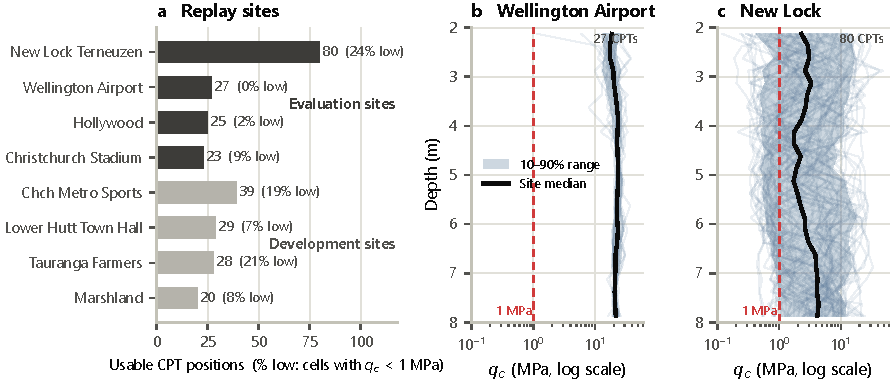
\includegraphics[width=\linewidth]{fig02_dataset.pdf}
\caption{Replay sites and profiles. (a)~Usable CPT positions at the eight replay sites and their share of
low cells ($\qc<1$\,MPa). (b,~c)~All 2--8\,m profiles at the most uniform (Wellington Airport) and most
variable (New Lock) evaluation sites. The band is the 10--90\% range and the black line the site median;
the $x$-axis is logarithmic.}
\label{fig:data}
\end{figure}
